% =============================================================================
%  Aetheric Geometry - technical report
%  Build:  pdflatex -interaction=nonstopmode AethericGeometry.tex   (run twice)
%  Requires only standard packages shipped with MiKTeX / TeX Live.
% =============================================================================
\documentclass[a4paper,10pt,twocolumn]{article}

\usepackage[utf8]{inputenc}
\usepackage[T1]{fontenc}
\usepackage{lmodern}
\usepackage[english]{babel}
\usepackage[margin=1.9cm,columnsep=0.7cm]{geometry}
\usepackage{amsmath,amssymb}
\usepackage{graphicx}
\usepackage{booktabs}
\usepackage{microtype}
\usepackage{caption}
\usepackage{titlesec}
\usepackage{xcolor}
\usepackage[colorlinks=true,linkcolor=black,citecolor=black,urlcolor=blue!55!black]{hyperref}

\graphicspath{{../analysis/figures/}}

\captionsetup{font=small,labelfont=bf,skip=4pt}
\titleformat{\section}{\normalfont\large\bfseries}{\thesection}{0.6em}{}
\titleformat{\subsection}{\normalfont\normalsize\bfseries}{\thesubsection}{0.6em}{}
\titlespacing*{\section}{0pt}{1.4ex plus .3ex}{0.8ex}
\titlespacing*{\subsection}{0pt}{1.1ex plus .2ex}{0.6ex}

\newcommand{\code}[1]{\texttt{\small #1}}

% -----------------------------------------------------------------------------
\begin{document}

\title{\vspace{-1.2em}\textbf{\LARGE Aetheric Geometry}\\[0.4em]
\large A gesture- and voice-controlled additive instrument:\\
design, signal processing, and measured corrections}

\author{Llu\'is Estap\'e\\
\small Universitat Polit\`ecnica de Catalunya\\
\small \href{mailto:lluis.estape@estudiantat.upc.edu}
            {lluis.estape@estudiantat.upc.edu}}

\date{}

\maketitle

\begin{abstract}
\noindent\small
Aetheric Geometry is a real-time instrument played with bare hands in front of
a webcam. Hand landmarks are reduced to a polygon whose geometry drives an
additive synthesiser tuned in just intonation, and a bilingual offline speech
layer freezes a sound and lets its effects be adjusted by turning a hand as one
would turn a knob. This report documents the system as built, but its subject
is narrower than that: it is an account of what measurement found in code that
already worked. A phase accumulator that looked correct was detuning every note
by $-3.385$ cents and emitting a glitch at 86.13\,Hz; a reverberator whose four
comb filters shared one feedback gain decayed at four different rates; a
waveform morph collapsed by 14\,dB in the middle of its travel through phase
cancellation; and a speech layer with a relaxed threshold fired six mutually
contradictory commands from one sentence. Each is derived analytically,
measured, corrected, and re-measured. The instrument runs its audio callback at
10.5\,\% of the deadline and its interface at 7.5\,ms per frame.
\end{abstract}

% =============================================================================
\section{Introduction}

The instrument occupies a lineage that predates its technology: instruments
played by moving the body through a field rather than by touching a key. What
the camera changes is not the idea but its cost. A webcam and a hand-landmark
model give twenty-one three-dimensional points per hand at video rate, and the
design question becomes what to do with them.

Aetheric Geometry answers it with a deliberately literal mapping. Two hands
pinch to open a \emph{thread} whose length sets pitch; pinching further fingers
adds vertices to a \emph{polygon} whose centroid, area, and aspect ratio drive
pitch, filter, reverberation, and tremolo. The polygon is not a metaphor. It
is a figure with measurable properties, and each property is bound to one
parameter, so the player can predict the sound from the shape.

Two additions turn this from a demonstration into something playable. The first
is \emph{hold}: a spoken word freezes the sounding chord, releasing the hands
from the job of maintaining it, after which they operate a virtual rotary
control. The second is a bilingual offline voice layer that accepts either
isolated commands or whole sentences. Both are described in
Sections~\ref{sec:hold} and~\ref{sec:voice}.

The system runs entirely offline: no network, no cloud speech, no external
audio engine. It ships as a Windows desktop application.

% =============================================================================
\section{How the project began, and what changed}

The instrument existed before this work in a form that was already complete as
a piece of interaction design. The gesture pipeline, the state machine, the
polygon mapping, and the visual language were all in place and behaved as
intended. What it lacked was any evidence that its signal processing did what
its own source comments claimed.

That distinction matters because none of the defects reported here announced
themselves. The instrument made sound; the sound was recognisably the sound
intended. The faults were found by writing down what each block was supposed to
compute, computing it, and comparing:

\begin{itemize}\itemsep2pt
\item The oscillator bank was detuned by a constant $-3.385$ cents and emitted a
      periodic discontinuity at 86.13\,Hz (Sec.~\ref{sec:phase}).
\item Sawtooth and square waves were generated without band limiting, aliasing
      at $-12$\,dB relative to signal at 2\,kHz (Sec.~\ref{sec:blep}).
\item The reverberator's four comb filters shared a single feedback gain,
      giving a 13.7\,\% spread in decay time, and had no diffusion stage
      (Sec.~\ref{sec:reverb}).
\item Envelope times were stored as raw one-pole coefficients, so every
      envelope changed with the device sample rate.
\item Just-intonation ratios were stored as rounded decimals
      (Sec.~\ref{sec:tuning}).
\item MIDI note numbers were emitted an octave flat.
\end{itemize}

The work also added the hold-and-knob layer, the voice layer, a continuous
waveform morph, MIDI output, a rebuilt interface, and a test suite that now
stands at 195 cases. Table~\ref{tab:modules} summarises the resulting
structure.

\begin{table}[t]
\centering\small
\begin{tabular}{@{}lrl@{}}
\toprule
Module & Lines & Responsibility \\
\midrule
\code{dsp.py}        & 290 & Oscillators, filters, delay lines \\
\code{synth.py}      & 421 & Engine, voicing, hold \\
\code{tuning.py}     & 124 & Exact ratios, pitch mapping \\
\code{knob.py}       & 221 & Rotary control geometry \\
\code{voice.py}      & 377 & Bilingual recognition, triage \\
\code{vocabulary.py} & 217 & Per-language word tables \\
\code{ui.py}         & 425 & Typography, panels, compositing \\
\code{renderer.py}   & 451 & Gesture overlay and HUD \\
\code{midiout.py}    & 191 & CC / pitch-bend output \\
\code{main.py}       & 450 & Event loop, state machine \\
\midrule
\code{tests/}        & 1190 & 195 cases \\
\bottomrule
\end{tabular}
\caption{Module structure. \code{dsp}, \code{tuning}, \code{knob} and
\code{vocabulary} have no camera, audio, or model dependencies, which is what
makes the numeric core testable and measurable without hardware.}
\label{tab:modules}
\end{table}

% =============================================================================
\section{Mapping geometry to sound}

\subsection{Pitch}

Pitch perception is logarithmic in frequency, so a linear map from hand
position would leave the low end musically cramped. The control value
$t\in[0,1]$ is mapped exponentially,
\begin{equation}
f(t) = f_{\text{lo}}\left(\frac{f_{\text{hi}}}{f_{\text{lo}}}\right)^{t},
\end{equation}
which gives constant cents per unit of hand travel. The result is then snapped
to the nearest degree of an A minor pentatonic scale, so that a moving hand
produces a playable line rather than a continuous glide.

\subsection{Just intonation, and its limit}
\label{sec:tuning}

Chords are built from exact rational ratios above the root, stored as
\code{Fraction} rather than as decimals. This is not pedantry. The point of
just intonation is that partials of different voices coincide \emph{exactly},
so that beating between them vanishes, and rounding destroys precisely that
property. The perfect fourth had been stored as $1.333$; against the true
$4/3$ the error is
\begin{equation}
1200\log_2\!\left(\frac{1.333}{4/3}\right) = -0.433\ \text{cents},
\end{equation}
inaudible as pitch, but not as beating: a fourth above 220\,Hz is 293.333\,Hz
exact and 293.260\,Hz rounded, and the third partial of the root then beats
against the second partial of the fourth at roughly 0.15\,Hz --- a slow wow
across a sustained chord, which is the artefact just intonation exists to
remove.

The system is honest about its own boundary. These are fixed ratios above a
\emph{movable} root, and the root is quantised to equal temperament. The
instrument is therefore justly tuned within a chord and equal-tempered between
chords. A fully just system has no single answer for what happens when the root
moves, because stacking exact fifths never closes the octave: twelve of them
overshoot by the Pythagorean comma,
\begin{equation}
1200\log_2\frac{(3/2)^{12}}{2^{7}} = 23.460\ \text{cents}.
\end{equation}
Choosing a fixed ratio set over a tempered root avoids comma drift at the cost
of transposition purity.

% =============================================================================
\section{The synthesis engine}

\subsection{A phase accumulator that was one sample short}
\label{sec:phase}

The oscillator rendered a block by forming a phase ramp and then storing the
phase back for the next block. It stored the phase of the \emph{last sample
rendered} rather than the phase the next block should \emph{begin} on. With a
block of $N$ samples the oscillator therefore advanced $N-1$ increments where
it owed $N$.

Two consequences follow. The effective frequency is scaled by $(N-1)/N$, a
constant detuning of
\begin{equation}
1200\log_2\frac{N-1}{N} = -3.385\ \text{cents}\quad (N = 512),
\end{equation}
and one sample of phase is replayed at every block boundary, producing a
discontinuity repeating at $f_s/N = 86.13$\,Hz. Measurement confirms both: the
nominal 440\,Hz tone appears at 439.08\,Hz before the fix and 440.09\,Hz after
(bin resolution 0.34\,Hz), and sidebands appear at $\pm 86$\,Hz around the
carrier.

\begin{figure}[t]
\centering
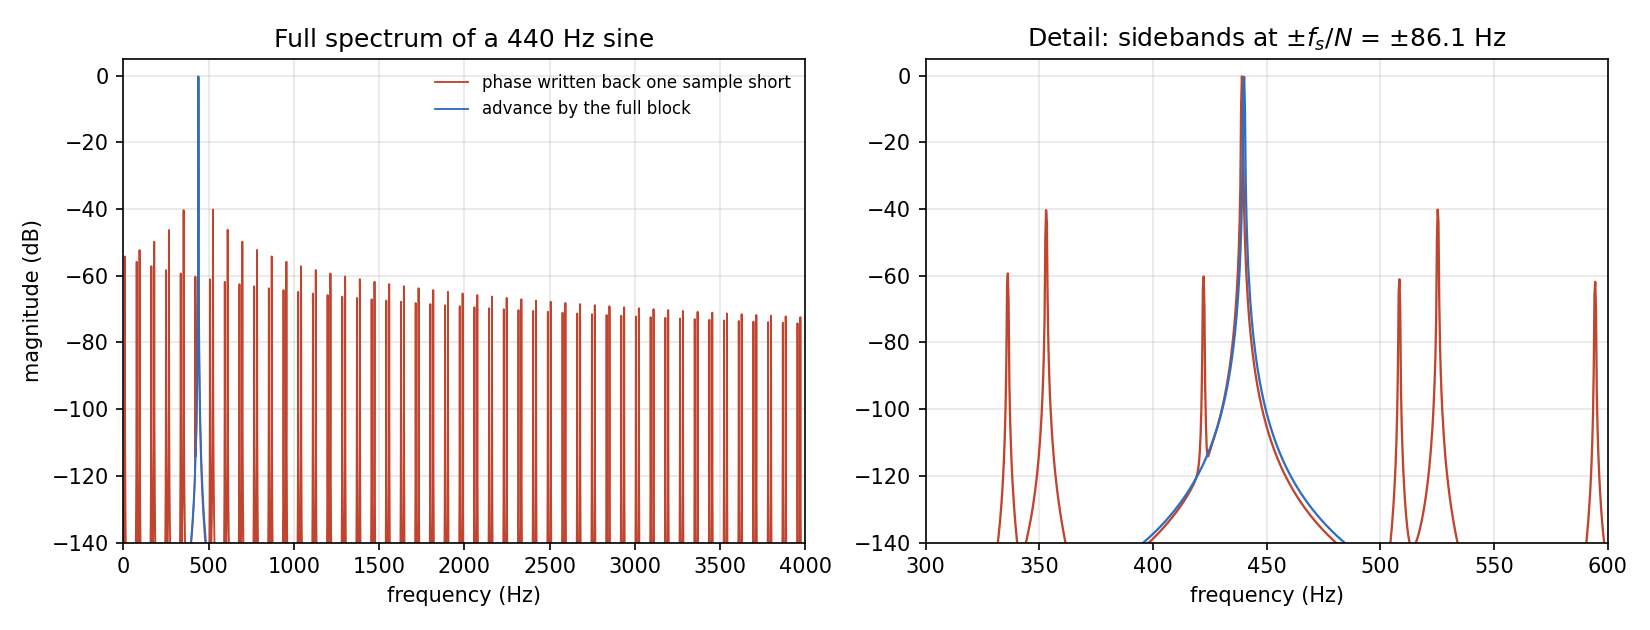
\includegraphics[width=\columnwidth]{phase_bug.png}
\caption{A 440\,Hz sine rendered by both accumulators. Left: full spectrum.
Right: detail around the carrier, showing the sidebands at $\pm f_s/N =
\pm 86.1$\,Hz produced by replaying one sample of phase per block.}
\label{fig:phase}
\end{figure}

The irony is worth stating. In an instrument built around exact frequency
ratios, every note was globally 3.4 cents flat with an 86\,Hz buzz on top ---
and because the error scales all partials equally, the ratios themselves
survived, which is exactly why nothing sounded obviously wrong.

\subsection{Band limiting}
\label{sec:blep}

A trivially generated sawtooth has harmonics at every multiple of $f_0$ with
amplitude $1/k$; all those above $f_s/2$ fold back as inharmonic partials. In
an instrument whose pitch is a continuous function of hand position the aliases
slide as the hand moves, which is far more noticeable than static aliasing on a
fixed note.

PolyBLEP replaces the discontinuity with a two-sample polynomial approximation
of a band-limited step. Writing $\phi$ for normalised phase and
$\Delta = f_0/f_s$, the residual subtracted at the wrap is
\begin{equation}
r(\phi) =
\begin{cases}
2u - u^2 - 1, & u = \phi/\Delta,\ \phi < \Delta,\\[2pt]
u^2 + 2u + 1, & u = (\phi-1)/\Delta,\ \phi > 1-\Delta,\\[2pt]
0 & \text{otherwise.}
\end{cases}
\end{equation}
The square wave applies the same residual at both edges; the triangle is
obtained by integrating the band-limited square with a leaky integrator whose
pole sits at $e^{-2\pi f_{\text{leak}}/f_s}$.

\begin{figure}[t]
\centering
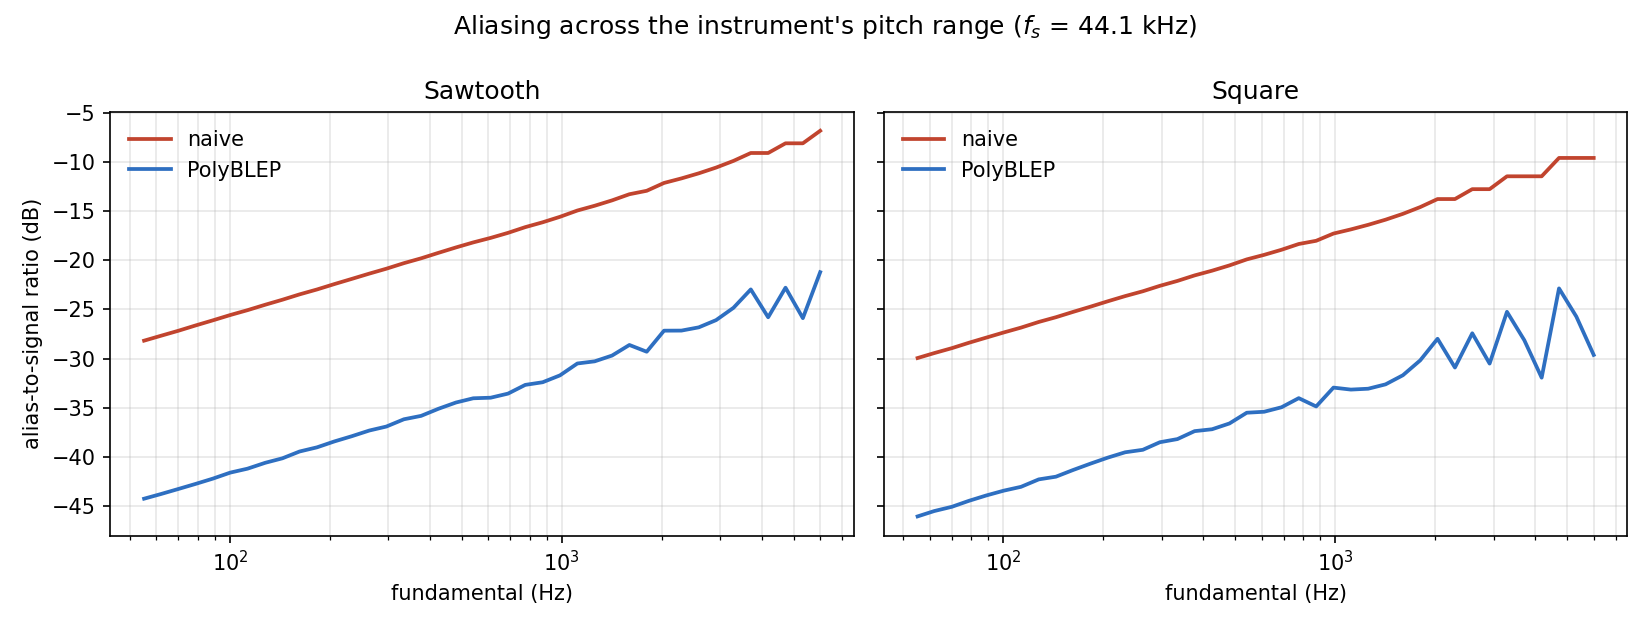
\includegraphics[width=\columnwidth]{aliasing_sweep.png}
\caption{Alias-to-signal ratio across the instrument's pitch range. Each
fundamental is placed on an exact FFT bin, so every true harmonic lands on a
bin and any off-grid energy is aliasing --- no window is needed and none is
applied.}
\label{fig:alias}
\end{figure}

Figure~\ref{fig:alias} shows the result. The correction buys a consistent
$\approx 16$\,dB: at 2031\,Hz the sawtooth improves from $-12.1$\,dB to
$-27.2$\,dB, and the square from $-13.8$\,dB to $-28.0$\,dB.

Measuring this required one methodological decision that carried more weight
than the correction itself. Each test fundamental is snapped to an exact FFT
bin, so that all harmonics fall on bins. With no spectral leakage, energy off
the harmonic grid \emph{is} aliasing, with no windowing assumption to defend.

\subsection{A prewarped filter}

The lowpass had used the naive one-pole $c = e^{-2\pi f_c/f_s}$, which is
accurate only while $f_c \ll f_s$. The topology-preserving-transform form uses
$g = \tan(\pi f_c/f_s)$ and $G = g/(1+g)$, collapsing to
\begin{equation}
y[n] = G\,x[n] + G\,x[n-1] + (1-2G)\,y[n-1],
\end{equation}
which is the bilinear transform of $1/(1+s/\omega_c)$ with frequency
prewarping. Unity gain at DC and an exact zero at Nyquist follow by substituting
$z=1$ and $z=-1$. Measured, the TPT form sits at $-3.010$\,dB at every
requested cutoff from 100\,Hz to 20\,kHz; the naive form drifts to $-0.987$\,dB
at 20\,kHz, a 2\,dB error.

\subsection{A reverberator that decayed four ways}
\label{sec:reverb}

The reverberator is a bank of four parallel feedback combs followed by allpass
diffusers. A comb of delay $D$ and gain $g$ emits echoes every $D/f_s$ seconds,
the $n$-th attenuated by $g^n$. Reaching $-60$\,dB requires $g^n = 10^{-3}$,
hence
\begin{equation}
T_{60} = \frac{-3D}{f_s \log_{10} g}
\qquad\Longleftrightarrow\qquad
g = 10^{-3D/(f_s T_{60})}.
\label{eq:rt60}
\end{equation}

The original code gave all four combs the same $g = 0.82$. By
Eq.~\eqref{eq:rt60} that makes $T_{60}$ proportional to $D$, and with delays
$\{1557, 1617, 1491, 1422\}$ the bank decays over $1.122$--$1.276$\,s: a
13.7\,\% spread, heard as a tail that comes apart rather than fading as one
object. Solving the right-hand form of Eq.~\eqref{eq:rt60} per comb from a
single $T_{60}$ target ties them together; measured decay then matches the
target to three decimal places.

\begin{figure}[t]
\centering
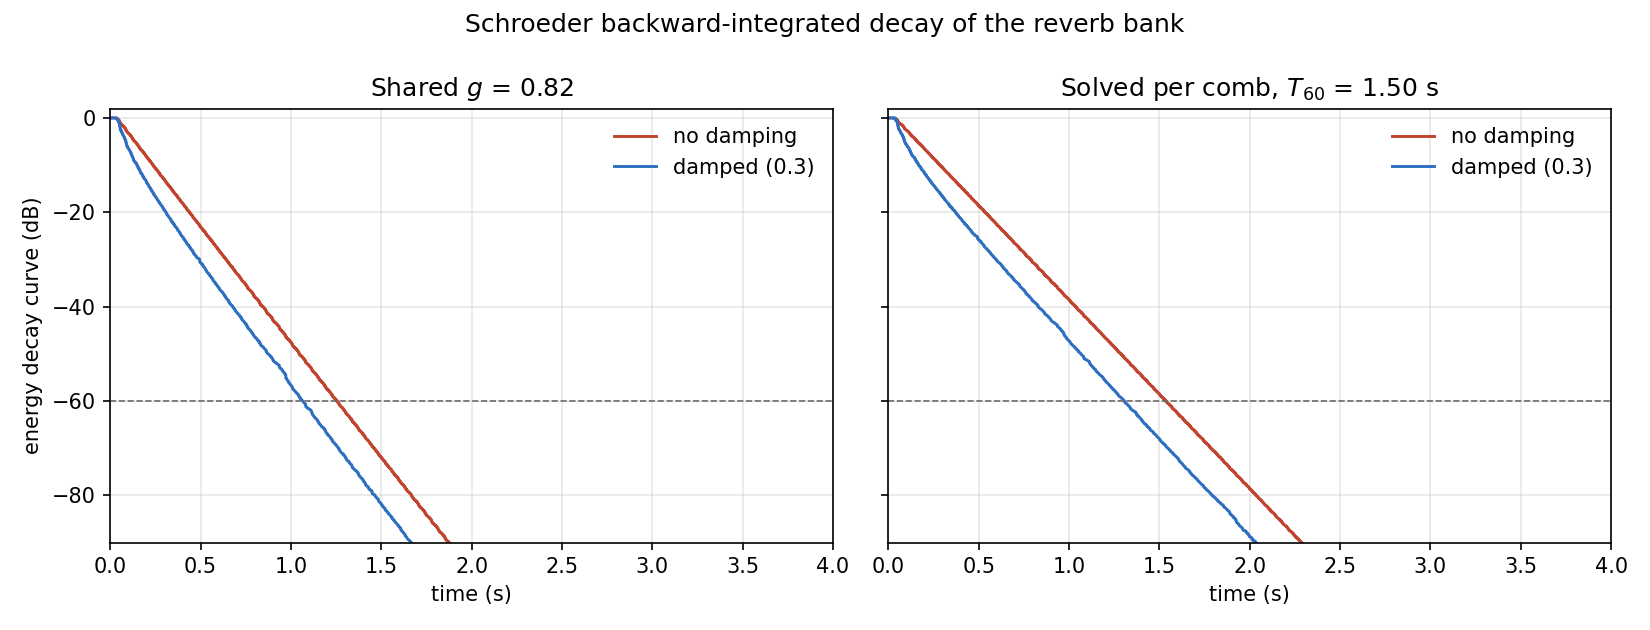
\includegraphics[width=\columnwidth]{reverb_decay.png}
\caption{Schroeder backward-integrated energy decay. Left: one shared feedback
gain. Right: per-comb gains solved from a single $T_{60}$ target.}
\label{fig:reverb}
\end{figure}

Two further corrections were made. Allpass diffusers of the canonical
single-delay-line form
\begin{equation}
H(z) = \frac{-g + z^{-D}}{1 - g z^{-D}},\qquad |H(e^{j\omega})| = 1,
\end{equation}
were added after the comb bank: the combs set the decay, the allpasses set
echo density. And a one-pole lowpass was placed inside each comb's feedback
path, making $T_{60}$ frequency-dependent so that high partials die first, as
they do in a room.

\subsection{Continuous waveform morph}

The four waveforms are the integer stops of one continuous control, ordered by
harmonic content --- sine, triangle, sawtooth, square --- so that the knob
behaves as a single edge control. Intermediate positions crossfade the two
neighbours; both are band limited and share a phase accumulator, so their sum
is band limited too.

The first implementation was unusable, and the reason is instructive. Measured
across the sweep, the sawtooth-to-square segment collapsed to an RMS of
$0.188$ against endpoints of $0.574$ and $0.995$ --- roughly 14\,dB down,
audible as the volume dropping out mid-travel. The cause is phase: a rising
ramp is negative through the first half of a cycle while a square is positive
through it, so mixing them subtracts.

The fix is to align the fundamental phase of all four shapes, which is
invisible on any shape alone --- inverting a sawtooth or shifting a triangle by
a quarter cycle is inaudible in isolation --- but is the difference between a
morph that works and one that does not. After alignment the sweep is monotone
in character and spans $0.54$ to $1.00$ RMS, which is the genuine loudness
difference between a triangle and a square rather than a defect.

% =============================================================================
\section{Hold and the rotary hand control}
\label{sec:hold}

Saying \emph{hold} freezes the sounding chord. The engine's \code{set\_params}
becomes a no-op while held --- that is what held \emph{means}, the hands stop
driving pitch and level --- while \code{set\_effect} continues to apply.

The freed hands then operate a rotary control. Pinching grips it; rotating the
hand in the camera plane turns it; releasing the pinch lets go while retaining
the value, so the arm can be repositioned and the turn continued. Rotation
accumulates, giving unlimited travel.

Two design decisions came from discarding something that did not survive
contact with a webcam. An earlier version used a flat palm facing the ceiling,
moved vertically; a palm facing the ceiling is nearly edge-on to the lens, its
landmarks are badly conditioned, and the grip flickered. Rotation about the
camera axis is the opposite: it is the most visible thing a hand can do, and
the wrist-to-knuckle vector that measures it is long and well separated from
the noise floor.

Second, finger extension is measured radially --- tip-to-wrist distance divided
by palm width --- rather than by comparing a fingertip's $y$ against its
knuckle's. The vertical test assumes an upright hand, and this gesture
\emph{rotates} the hand, which is precisely when that assumption fails.
Normalising by palm width also makes the measure invariant to distance from the
camera.

Angles are unwrapped to $[-\pi,\pi]$ before accumulation. This imposes a
sampling limit worth naming: a rotation of more than half a revolution between
two video frames is indistinguishable from a smaller one in the opposite
direction. This is the Nyquist criterion applied to angle; at 30\,fps it allows
15 revolutions per second and never binds in practice.

% =============================================================================
\section{Voice control}
\label{sec:voice}

Speech recognition is offline (Vosk), with English and Spanish models running
\emph{in parallel} on one microphone stream. This is not a preference. An
acoustic model is language-specific: \emph{hold} is absent from the Spanish
lexicon and \emph{congela} from the English one, and a constrained grammar may
only contain words its model already knows. Decoding twice is the only way to
hear both.

The layer performs keyword spotting, not parsing. A result is scanned word by
word and anything in the vocabulary fires; \emph{vamos a probar una onda
cuadrada} works because \emph{cuadrada} is in it, not because the sentence was
understood. Ordinary sentence glue --- articles, pronouns, verbs of request ---
is included in the grammar but mapped to nothing, because a closed grammar is
closed: every sound reaching it lands on \emph{some} entry, and without
somewhere harmless to put the other five words of a sentence they smear across
the words that are commands.

\subsection{Four gates, each from a measurement}

\begin{table}[b]
\centering\small
\begin{tabular}{@{}llr@{}}
\toprule
Gate & Question & Without it \\
\midrule
Final results only & utterance done?   & 11 cmds / 25\,s \\
Peak RMS level     & did anyone speak? & 1 cmd / 45\,s \\
Length triage      & meant for us?     & 11 cmds / 40\,s \\
One per family     & which intent?     & 6 per sentence \\
\bottomrule
\end{tabular}
\caption{Each gate answers a different question, and each was added after
measuring the failure that motivated it. Counts are spurious commands observed
in ordinary room conditions with nobody addressing the instrument.}
\label{tab:gates}
\end{table}

Table~\ref{tab:gates} lists them. Two deserve explanation.

\textbf{Level, not confidence.} A constrained grammar assigns room tone to its
nearest listed word, sometimes at high confidence: 45\,s of silence produced a
command at confidence $0.87$. Confidence answers \emph{which word is this most
like}, never \emph{was anyone speaking}. Speech into a laptop microphone runs
an order of magnitude above room tone, so peak RMS answers the second question
cleanly.

\textbf{Length triage.} Requiring a wake word for everything makes the
instrument unusable --- short commands must work mid-performance with no
ceremony --- while requiring nothing lets room conversation play the
instrument. Length decides: utterances of three words or fewer fire bare;
longer ones require the wake word \emph{aether} and are otherwise dropped
whole. Measured, ordinary conversation produced 11 spurious commands in 40\,s
without triage and none with it.

\subsection{One intent per family}

The last gate is the subtlest. Inside a phrase that followed the wake word,
per-word confidence is judged more leniently, because connected speech scores
far lower than an isolated word and a single strict threshold accepted
\emph{eco} alone while silently dropping the identical word inside a sentence
--- which reads, from outside, as the wake word working and the sentence being
ignored.

That leniency then produced a new failure. A single utterance was logged
emitting \code{wave:SIN}, \code{release}, \code{hold}, \code{select:reverb},
\code{wave:SQUARE} and \code{wave:TRIANGLE} within four milliseconds. The last
one wins and the instrument appears to ignore the request.

The correction groups candidates by intent family --- a selection, a waveform,
a relative move, a hold --- and fires the best-scoring word in each. Words
within a family are alternatives; families are independent, so
\emph{aether, take the echo and lower it thirty percent} legitimately means two
things and does both. Mutually exclusive families (hold against release) resolve
to the higher confidence.

Spoken numbers are read as percentages, since Vosk emits words rather than
digits and \emph{treinta por ciento} must be looked up rather than parsed.

% =============================================================================
\section{Real-time behaviour}

\subsection{Audio}

A block of 512 frames at 44.1\,kHz must be produced within 11.61\,ms. Measured
over 400 blocks, the worst case --- eight partials, triangle waveform, every
effect engaged --- has a 95th-percentile cost of 1.22\,ms, or \textbf{10.5\,\%}
of the deadline.

That headroom is the product of one structural observation. A feedback comb
\code{y[n] = x[n] + g\,y[n-D]} looks like a sequential recursion, but when $D$
is at least the processing chunk length, every sample it reads was written
before the current chunk began. The recursion then unrolls into a delay-line
read and a vector multiply. Splitting each block at the delay-line wrap
guarantees that condition, which is what allows four combs and two allpasses to
run in a Python callback without a per-sample loop.

\subsection{Interface}

The overlay is drawn with real typefaces through Pillow rather than OpenCV's
Hershey fonts. Rendered naively it cost 39\,ms per frame. Three changes brought
that to 4.6--7.5\,ms:

\begin{itemize}\itemsep2pt
\item Rasterised tiles are cached against their content, so most frames become
      a composite rather than a redraw.
\item Channel order and float promotion are done once at rasterise time rather
      than per frame; the composite alone fell from 5.9\,ms to 1.4\,ms.
\item The effects panel is split into three tiles by how fast each changes, so
      turning a control redraws a dial rather than a panel.
\end{itemize}

One defect here is worth recording because it was invisible: the effect-meter
loop used \code{key} as its loop variable, shadowing the cache key computed
above it. Tiles were stored under the wrong key and the cache never hit. The
panel looked correct and simply ran at full cost indefinitely.

Camera frames are resampled to the display size \emph{before} the overlay is
drawn. Many webcams deliver only 1920$\times$1080 and ignore requests for
anything smaller, and letting the window rescale the finished frame resampled
rendered text by an arbitrary ratio --- the operation that makes type look
chewed, and one no amount of better typography survives.

% =============================================================================
\section{Output and packaging}

Effect values, pitch, and note state are mirrored as MIDI, which turns the
whole gesture and voice surface into a general-purpose controller: the internal
engine becomes the demonstration and the control surface becomes the product.
Values are quantised to the 0--127 that a control change actually carries and
compared against the last value sent; pitch is sent as one held note plus pitch
bend rather than as a note per semitone, because retriggering per semitone on a
continuous pitch would sound like a machine gun.

Two properties were measured through a loopback port
(\code{analysis/measure\_midi.py}). \textbf{Transport delay}, timed by opening
the same virtual cable as both output and input and pairing each message with
its arrival, has a median of 5.65\,ms (min 5.01, p95 6.32, 200/200 delivered).
Timing \code{send()} alone would have measured the call returning rather than
the message arriving, which is a different and much smaller number. That figure
is an upper bound rather than pure driver cost, since it includes Python thread
scheduling on the receiving side --- but it is the bound that matters, because
it sits on a pipeline whose dominant term is the 33\,ms video frame period. The
transport is not what the player feels.

\textbf{Traffic} confirms the send-on-change design rather than asserting it. A
still hand held for 120 frames emitted \textbf{zero} messages. Six controls
swept simultaneously --- far beyond what one pair of hands can do --- emitted
163 messages per second, or 15.7\,\% of the roughly 1041 three-byte messages
per second a MIDI 1.0 stream carries. The rate limiter therefore never binds in
practice, and the automation a DAW records is continuous rather than stepped.

\subsection{Reaching a host}

Windows provides no virtual MIDI port of its own, so the loop is closed with
loopMIDI. Output was confirmed arriving in FL Studio, which plays notes sent
down the cable through whichever generator is selected.

Two practical findings are worth recording because both cost time and neither
is documented anywhere obvious.

First, \textbf{the same virtual cable is not called the same thing on both
sides}. The rtmidi backend appends each port's ordinal \emph{within its own
direction's list}, so the output \code{loopMIDI Port 1} is the input
\code{loopMIDI Port 0}. Matching a loopback pair on the full string finds
nothing; the pairing has to be done on the name with its trailing index
stripped. This is exactly the kind of detail that makes a working cable look
broken.

Second, \textbf{a host's MIDI-learn latches onto the first control change it
sees}. Running the whole instrument to generate one moves six controls at once,
so the mapping lands on whichever message happened to arrive first --- rarely
the intended one, and tedious to undo. A dedicated tool
(\code{analysis/midi\_learn.py}) therefore sends a single CC on a slow
triangular sweep across the full 0--127 range: one control removes the
ambiguity, and the sweep gives the host a range to infer rather than a single
value it may miss between window redraws.

Diagnosis follows the same principle. \code{analysis/midi\_ping.py} sends notes
rather than control changes, on every loopback port in turn. Verifying a cable
with a control change requires finding an activity indicator in the host and
trusting it is the right one; notes need no indicator, because if the host is
receiving, the instrument plays and the result arrives through the ear. Walking
every port also separates \emph{is the cable working} from \emph{is the host
listening to this particular cable}, two questions a single-port test conflates
into one unhelpful silence.

The application is frozen with PyInstaller into a one-folder Windows build.
Two constraints shaped it. The bundle carries two speech models and MediaPipe's
graph data --- roughly 150\,MB --- so a single-file build would re-extract that
on every launch. And \code{matplotlib} cannot be excluded despite nothing in the
application plotting anything, because MediaPipe's drawing utilities import it
at module scope; excluding it to save 40\,MB produced a build that died on
\code{import mediapipe} behind a dialog reading only \emph{Unhandled exception
in script}.

% =============================================================================
\section{Limitations}

\textbf{Gesture and voice contend for three parameters.} While not held, the
polygon mapping rewrites filter, reverberation, and tremolo every frame, so a
spoken adjustment to those three is undone on the next video frame. The
remaining parameters are unaffected because no gesture writes them. The fix is
parameter ownership --- a value touched by voice should resist the gesture path
until released --- and is not yet implemented.

\textbf{The main loop is untested.} Every numeric module has unit coverage, but
the event loop, state machine, and rendering call sequence live in a single
450-line function with none. Extracting the state machine into a class would
make the core of the program testable.

\textbf{Typography is substituted.} The interface specifies Inter and IBM Plex
Mono; neither ships with Windows and a desktop build has nowhere to fetch a
webfont. The nearest installed equivalents are used instead.

\textbf{The end-to-end chain is not yet measured.} What has been timed is the
transport --- 5.65\,ms median from send to arrival --- and separately the video
and audio stages. What has not is the whole path from a hand moving to a mapped
parameter audibly changing in a host, which is the only figure a producer would
care about. It is a harder measurement than it sounds, because the endpoint is
acoustic: it needs the DAW's output recorded alongside a timestamped gesture,
with the host's own buffer and any parameter smoothing included in the total.
Until that exists, the honest statement is that each stage is small and the sum
has not been demonstrated.

% =============================================================================
\section{Conclusion}

The instrument works, and worked before this study began. What the study adds
is the difference between an instrument that sounds right and one that can be
shown to be right. Every correction reported here was found the same way: by
writing down what a block was supposed to compute, computing it, and comparing
--- and in every case the defect had been inaudible as a defect, presenting
instead as a slight dullness, a tail that came apart, a control that felt
uneven, or a voice command that seemed not to register.

The measurements are reproducible from the repository:
\code{analysis/measure\_dsp.py} regenerates every figure and number in
Sections 4 and 5, \code{analysis/measure\_midi.py} times the output transport
and counts its traffic, and \code{analysis/voice\_monitor.py} exposes the
speech layer's decisions word by word with confidence and level.

% =============================================================================
\section*{References}
\small
\begin{enumerate}\itemsep1pt
\item M.~R. Schroeder, ``Natural sounding artificial reverberation,''
      \emph{J. Audio Eng. Soc.}, vol.~10, no.~3, 1962.
\item V.~V\"alim\"aki and A.~Huovilainen, ``Antialiasing oscillators in
      subtractive synthesis,'' \emph{IEEE Signal Processing Magazine},
      vol.~24, no.~2, 2007.
\item V.~Zavalishin, \emph{The Art of VA Filter Design}, rev.~2.1.0, 2018.
\item T.~Stilson and J.~O. Smith, ``Alias-free digital synthesis of classic
      analog waveforms,'' \emph{Proc. ICMC}, 1996.
\item M.~Wright and D.~Wessel, ``Problems and prospects for intimate musical
      control of computers,'' \emph{Computer Music Journal}, vol.~26, no.~3,
      2002.
\end{enumerate}

\end{document}
